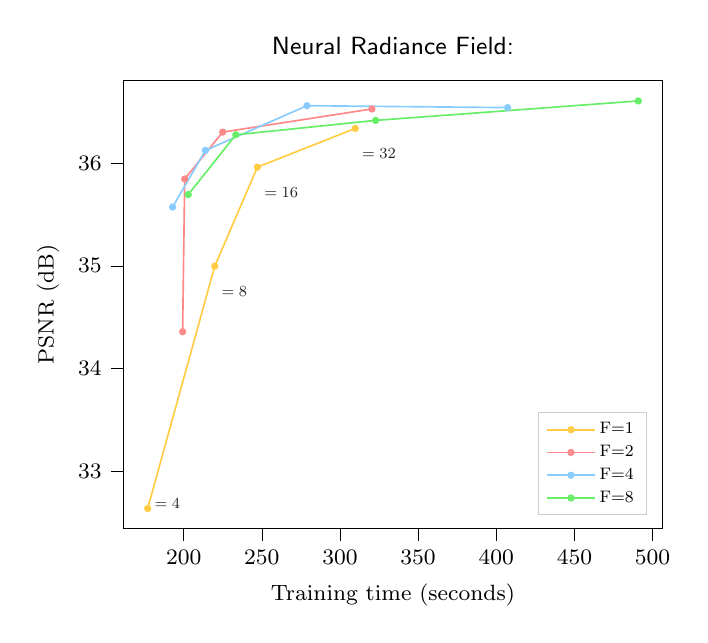
\begin{tikzpicture}
\tikzstyle{every node}=[font=\footnotesize]


\definecolor{color0}{rgb}{1,0.8,0.266666666666667}
\definecolor{color1}{rgb}{1,0.533333333333333,0.533333333333333}
\definecolor{color2}{rgb}{0.533333333333333,0.8,1}
\definecolor{color3}{rgb}{0.4,0.933333333333333,0.4}

\begin{axis}[
legend cell align={left},
legend style={
  fill opacity=0.8,
  draw opacity=1,
  text opacity=1,
  at={(0.97,0.03)},
  anchor=south east,
  draw=white!80!black,
  nodes={scale=0.75, transform shape}
},
tick align=outside,
tick pos=left,
title={{\small \sffamily Neural Radiance Field: \sceneLego}},
x grid style={white!69.0196078431373!black},
xlabel={Training time (seconds)},
xmin=161.283349061012, xmax=506.544362044334,
xtick style={color=black},
y grid style={white!69.0196078431373!black},
ylabel={PSNR (dB)},
ymin=32.4409293696302, ymax=36.8024791114829,
ytick style={color=black}
]
\addplot [semithick, color0, mark=*, mark size=1, mark options={solid}]
table {%
176.977031469345 32.6391816306235
219.887970209122 34.9971521778585
247.183665275574 35.9605496985434
309.770037174225 36.3368775803035
};
\addlegendentry{F=1}
\addplot [semithick, color1, mark=*, mark size=1, mark options={solid}]
table {%
199.329049110413 34.3594561463158
200.676287412643 35.8455825108642
224.979252815247 36.3012873233936
320.418728590012 36.5261911390268
};
\addlegendentry{F=2}
\addplot [semithick, color2, mark=*, mark size=1, mark options={solid}]
table {%
192.913296699524 35.572185179762
213.924275636673 36.1229185152962
278.900064468384 36.5581807548899
407.25347161293 36.539436401952
};
\addlegendentry{F=4}
\addplot [semithick, color3, mark=*, mark size=1, mark options={solid}]
table {%
202.953203201294 35.6939234735322
233.376142501831 36.2753909092502
322.851065158844 36.4151717077674
490.850679636002 36.6042268504896
};
\addlegendentry{F=8}
\draw (axis cs:176.977031469345,32.6391816306235) node[
  scale=0.7,
  anchor=base west,
  text=white!15!black,
  rotate=0.0
]{$\levels = 4$};
\draw (axis cs:219.887970209122,34.7013365018841) node[
  scale=0.7,
  anchor=base west,
  text=white!15!black,
  rotate=0.0
]{$\levels = 8$};
\draw (axis cs:247.183665275574,35.664734022569) node[
  scale=0.7,
  anchor=base west,
  text=white!15!black,
  rotate=0.0
]{$\levels = 16$};
\draw (axis cs:309.770037174225,36.0410619043291) node[
  scale=0.7,
  anchor=base west,
  text=white!15!black,
  rotate=0.0
]{$\levels = 32$};
\end{axis}

\end{tikzpicture}
